\documentclass[oneside,12pt]{article}
\usepackage[a4paper,width=150mm,top=25mm,bottom=25mm]{geometry}
\usepackage[utf8]{inputenc}
\usepackage[english]{babel}
\usepackage{graphicx}   \graphicspath{{figures/}}
\usepackage[margin=30pt,labelfont=bf,labelsep=period,font={small,stretch=1.1}]{caption} % Caption settings
\usepackage{setspace}
\usepackage[font={normal,stretch=1.1}]{subcaption}
\usepackage{amssymb,wasysym}% Symbols
% \usepackage[table,dvipsnames]{xcolor}     % Provides a common set of commands for color manipulation
\usepackage[hidelinks]{hyperref} % Links: table of contents, references, bibliography, figures, pages, url's, etc.
\usepackage{fancyhdr} \pagestyle{fancy} % Page heading
\fancyhead[L]{\nouppercase{\rightmark}} \fancyhead[R]{\nouppercase{\leftmark}} % No uppercase
\usepackage{array} % To control table cell width
\usepackage{makecell}
\usepackage[]{natbib} \bibliographystyle{apalike}    % Bibliography management
\usepackage{blindtext}
\usepackage{soul}
\usepackage{lscape}
\usepackage{color}
\usepackage{algpseudocode}
\usepackage{algorithm}
\newcommand{\un}[1]{\,\mathrm{#1}}
\algnewcommand{\LineComment}[1]{\State \(\triangleright\) #1}
\newcommand{\bigO}{\mathcal{O}}
\newcommand{\codeword}[1]{\texttt{\textcolor{blue}{#1}}}
\begin{document}

\setlength{\parindent}{0 em}    % Paragraph indentation
\setlength{\parskip}{0.7 em}    % Space between paragraph and preceding text
\renewcommand{\baselinestretch}{1.5}    % Line spacing

\newcommand{\ProjectTitle}{AMESP - Phase 2 WP3} % <---Write here the project title!!!

\begin{titlepage}
    \begin{center}
    \vspace*{3 cm}
    \Huge
    \textbf{Report} \\
    \vspace{1 cm}    
    \textbf{\ProjectTitle}
    \\
    \vspace{1 cm}
    \vfill      % Automatically add in the amount of vertical space needed for the content to fill the page
    
\includegraphics[width=60mm]{figures/NHLStenden-logo.png} \\
    \end{center}
    \vspace{2 cm}
    \normalsize
    Title : \ProjectTitle
    \\
    Authors : K. S. Moreira, Luewton L F Agostinho, R.H. Braga Leivas
    \\
    Date : \today 
    \\
    Code : 
    \\
    Version : 1 \\
    Status : draft \\
    Mailing list : 
    \\
    Copy to : \\
    Classification : confidential
\end{titlepage}

% \chapter*{} \thispagestyle{empty}   % "Page break"
% \chapter*{} \thispagestyle{empty}   % "Page break"

% ---------- MAIN TEXT ---------- %
\setlength{\parindent}{0 em}  % Paragraph indentation
\setlength{\parskip}{0.7 em}    % Space between paragraph and preceding text

\newpage    \pagestyle{empty}
\tableofcontents
\pagestyle{fancy}
\newpage

% ==============================================
% \newpage
\section{WP3 Overview}

\subsection{Objectives}

Based on the signed proposal, ... 

\subsection{Timeline of Executed Tasks}

\subsection{Conventions}

Throughout this section, we'll refer multiple times to physical variables of the system. \autoref{fig:setup-conventions}
shows the variable conventions we'll use in this text.

\begin{figure}[h!]
    \centering
    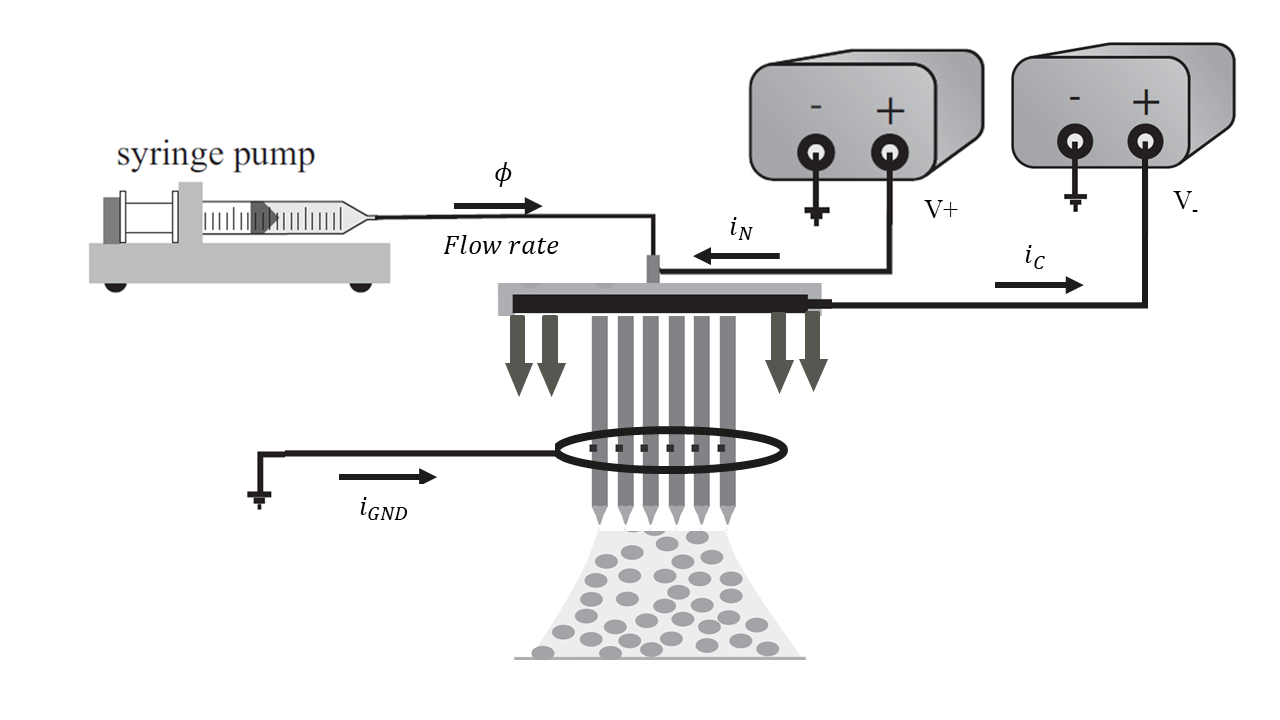
\includegraphics[width=.9\textwidth,trim=1 1 1 1,clip]{figures/setup-conventions.png}
    \caption{Variable conventions and nomenclature. Source: adapted from \cite{Verdoold2013}.}
    \label{fig:setup-conventions}
\end{figure}

As shown in \autoref{fig:setup-conventions}, we have

\begin{itemize}
    \item $i_N$: current flowing from the positive high voltage source to the nozzles
    \item $i_C$: current flowing from the crown to the negative high voltage source
    \item $i_{GND}$: current flowing from the ground to the ring
    \item $\phi$: flow rate of the syringe pump
    \item $V_+$: voltage of the positive high voltage
    \item $V_-$: voltage of the negative high voltage
\end{itemize}

The direction of the currents was chosen as shown in \autoref{fig:setup-conventions} to ensure they are always positve 
in the measurements, faciliting the analysis.


% ==============================================
% \newpage
\section{First Approach: PID Controller}

\subsection{Time Response Analysis}

Before developing a proof-of-concept PID controller for the multinozzle, we first 
need to understad the time resonse of system to changes in the input.

\begin{figure}[h!]
    \centering
    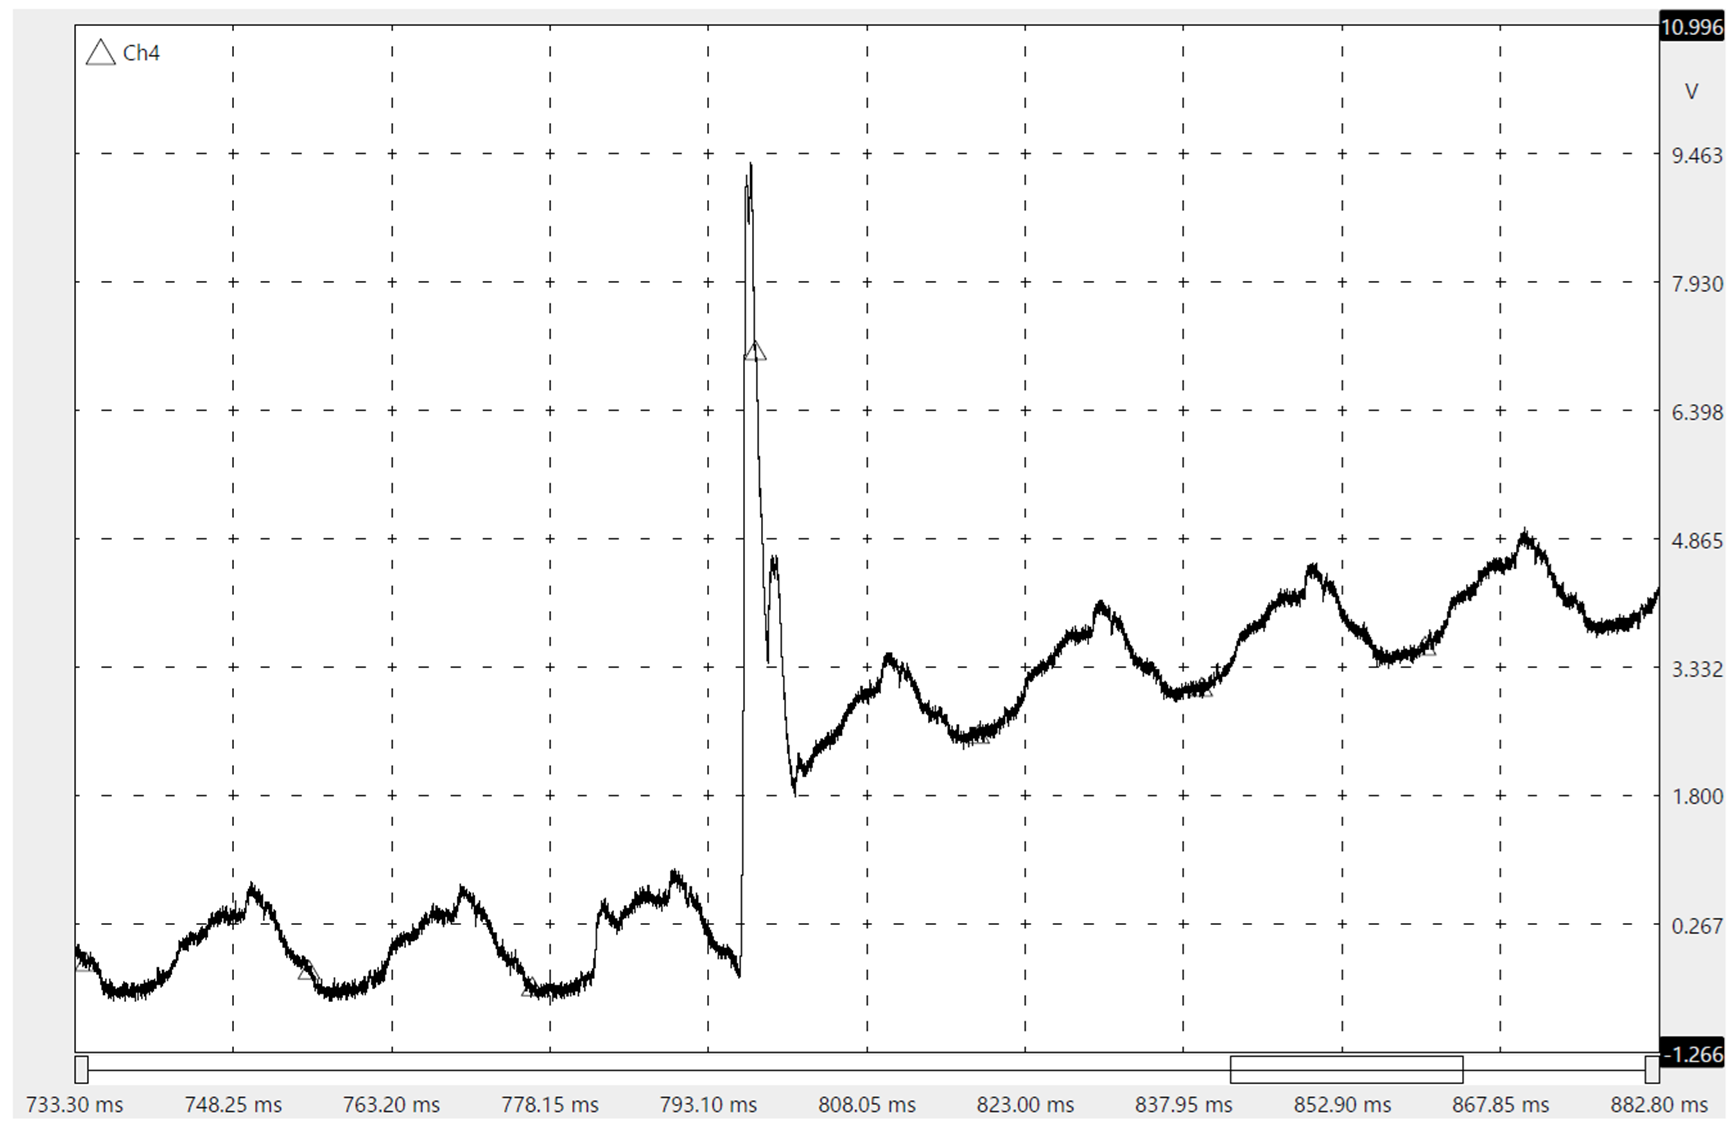
\includegraphics[width=.8\textwidth,trim=1 1 1 1,clip]{figures/inrush-current.png}
    \caption{Inrush current on the positive HV+ line.}
    \label{fig:inrush-current}
\end{figure}

\subsubsection{Subsubsection}

\blindtext % Remove this and write your text!

% ==============================================
% \newpage
\section{Second Approach: Current-based Classification and Control} 

Once identified the issues with the first approach, we attempted to design a 
controller based on the classification suggested by \cite{Verdoold2013}.

The strategy adopted will be to first classify the electrospray mode by looking a current values 
on the system, and then experimentally design a controller that can move from an intermittent
to a cone-jet spray mode.

However, Verdoold's method was designed for the single nozzle, and it is not clear if we can 
extend his classification to a multinozzle configuration. Therefore, part of this work 
includes an attempt to extend his classification to the system developed by 
Gilbert.


\subsection{Measuring the currents by spray mode}

The first test done was to measure the current on all three lines of the sprayhead and 
verify if we see a pattern in the shape of current that can be used to classify the spray mode.
\autoref{fig:setup-three-currents-spray-mode} shows the setup used for this test. $V_-$ was fixed on 
$V_- = - 4.5 kV$.

\begin{figure}[h!]
    \centering
    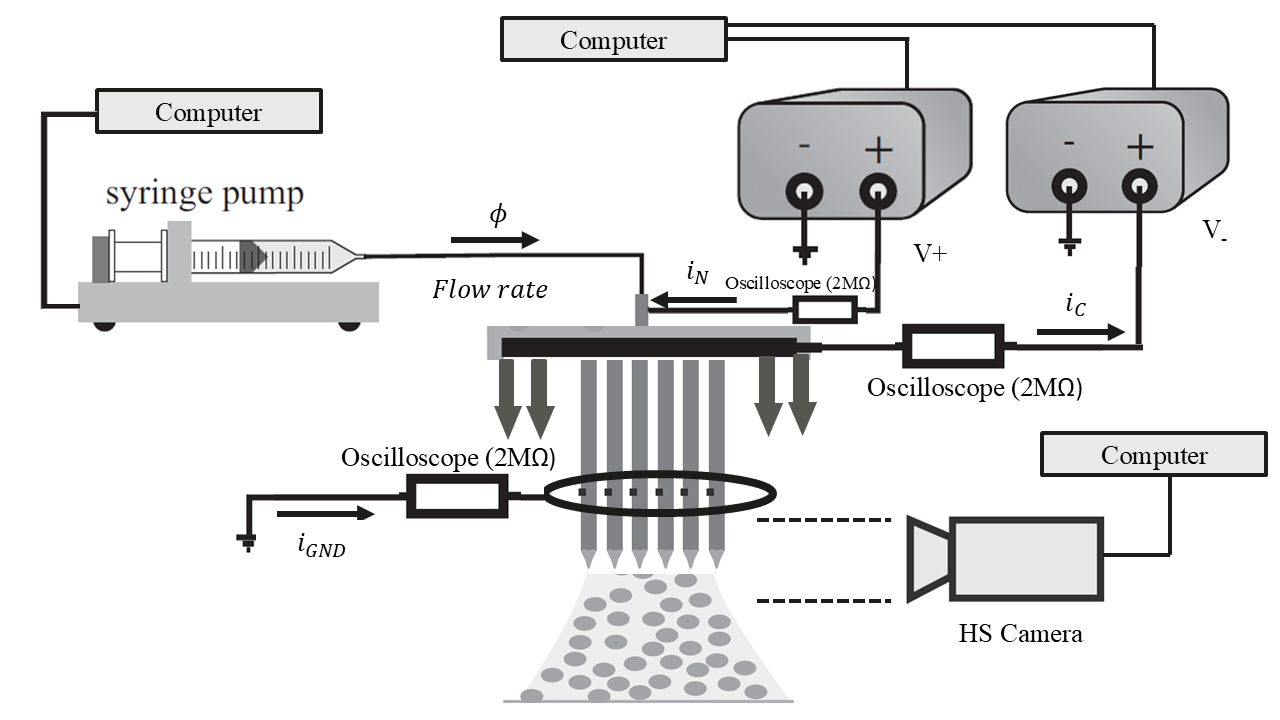
\includegraphics[width=.8\textwidth,trim=1 1 1 1,clip]{figures/setup-three-currents-spray-mode.png}
    \caption{Setup to measure all three currents on the sprayhead. Source: adapted from \cite{Verdoold2013}.}
    \label{fig:setup-three-currents-spray-mode}
\end{figure}

Using three oscilloscopes, all three currents were sampled at 5 kHz, collecting 20.000 samples of each
(totalling a 4 seconds time window). Notice that, although the oscilloscope has multiple channels, 
we cannot use the same oscilloscope as the channels are interconnected internally: the high voltage 
differences would damage the instrument. Therefore, we use one oscilloscope for each line. 

\autoref{fig:three-currents-spray-mode-50ms} and \autoref{fig:three-currents-spray-mode-500ms} show the waveforms 
obtained for $\phi = 20 \un{mL/h}; \phi = 30 \un{mL/h}; \phi = 50 \un{mL/h}$ for two different time windows: 50ms 
and 500ms.

\begin{figure}[h!]
    \centering
    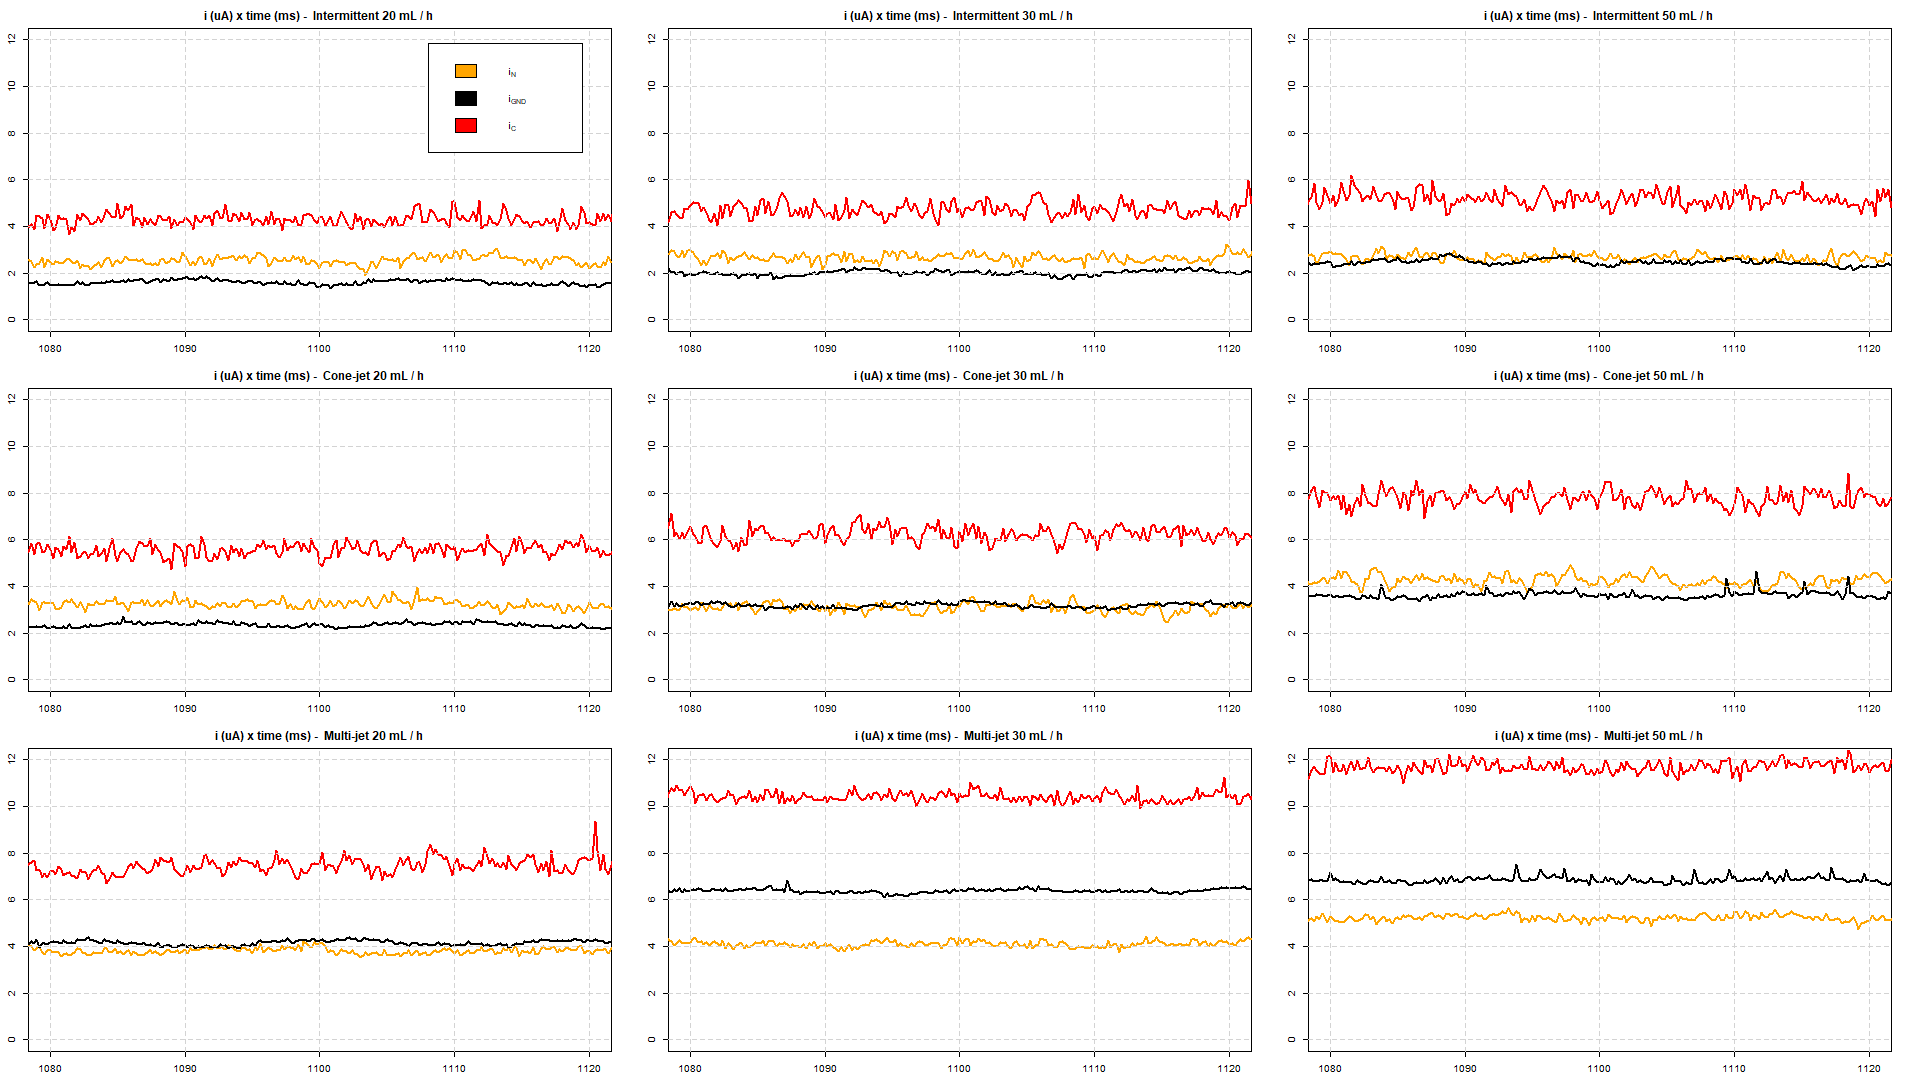
\includegraphics[width=1\textwidth,trim=1 1 1 1,clip]{figures/three-currents-spray-mode-50ms.png}
    \caption{$i_N$, $i_{GND}$ and $i_C$ over time by different spray modes - 50 ms time window.}
    \label{fig:three-currents-spray-mode-50ms}
\end{figure}

\begin{figure}[h!]
    \centering
    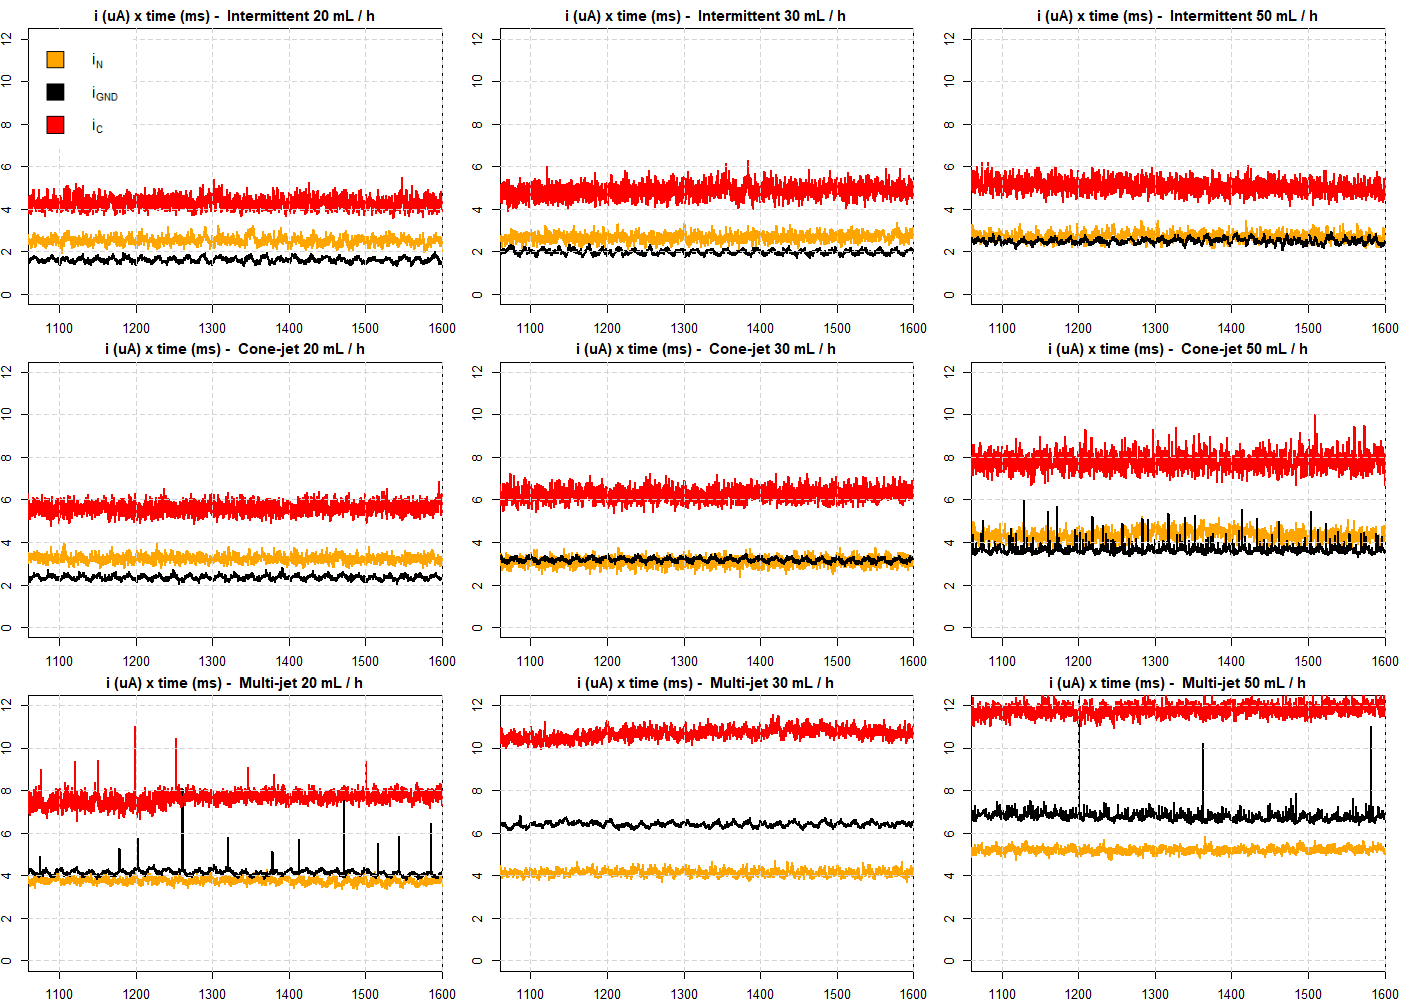
\includegraphics[width=1\textwidth,trim=1 1 1 1,clip]{figures/three-currents-spray-mode-500ms.png}
    \caption{$i_N$, $i_{GND}$ and $i_C$ over time by different spray modes - 500 ms time window.}
    \label{fig:three-currents-spray-mode-500ms}
\end{figure}

As we can see in \autoref{fig:three-currents-spray-mode-50ms} and \autoref{fig:three-currents-spray-mode-500ms}, 
we don't see a clear distinction in the shape of the current 
by different spray modes, in both time windows. The sharp peaks we see on the waveforms are most likely caused
by a high-frequency noise in signal, especially since we use banana adapters for the oscilloscope in this test, instead
of coaxial cables, which pick up less noise.

Attempting to see a distinction on \autoref{fig:three-currents-spray-mode-500ms} via the standard deviation also
fails, as shown on \autoref{fig:three-currents-spray-mode-sd}.

\begin{figure}[h!]
    \centering
    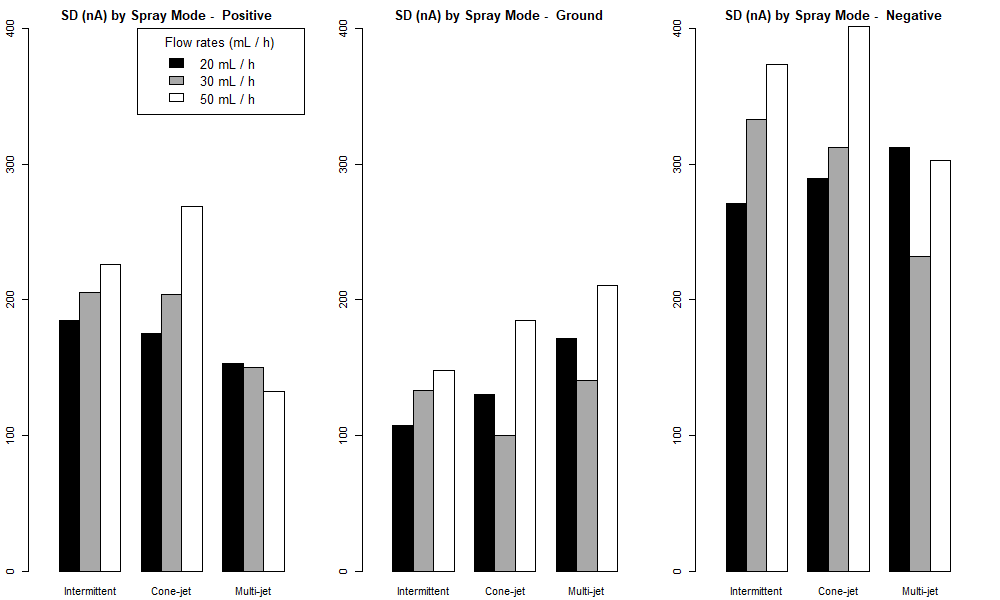
\includegraphics[width=1\textwidth,trim=1 1 1 1,clip]{figures/three-currents-spray-mode-sd.png}
    \caption{Standard deviation on \autoref{fig:three-currents-spray-mode-500ms} of $i_N$, $i_{GND}$ and $i_C$
    by spray mode.}
    \label{fig:three-currents-spray-mode-sd}
\end{figure}

Without a clear distinction in the current waveforms it would not possible to continue with this approach.
Therefore, we need to first understand why we are not seing distinctions in the shape 
of the current, particularly between the intermittent and cone-jet spray modes, as it is clear in the 
literature that there should be a difference.

To do this, we'll begin by attempting to reproduce \cite{Verdoold2013}'s results, with the goal of isolating 
if the problem is our measurement strategy or if it is something related to the sprayhead itself.

\subsection{Reproducing Results from \cite{Verdoold2013}}

\autoref{fig:verdoold-reproduce-setup} shows the setup used to reproduce \cite{Verdoold2013}'s approach.
We used a sampling frequency of 5 kHz and $\phi = 1 \un{mL/h}$. 

\begin{figure}[h!]
    \centering
    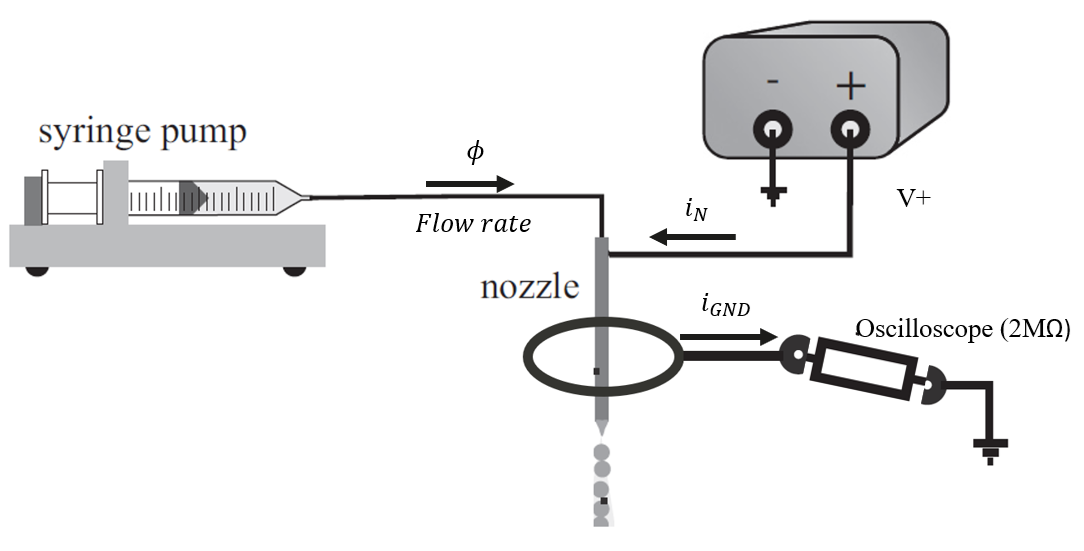
\includegraphics[width=.8\textwidth,trim=1 1 1 1,clip]{figures/verdoold-reproduce-setup.png}
    \caption{Setup used to reproduce Verdoold's classification method. Source: adapted from \cite{Verdoold2013}.}
    \label{fig:verdoold-reproduce-setup}
\end{figure}

The results obtained are shown in \autoref{fig:verdoold-reproduce-results}. 

\begin{figure}[h!]
    \centering
    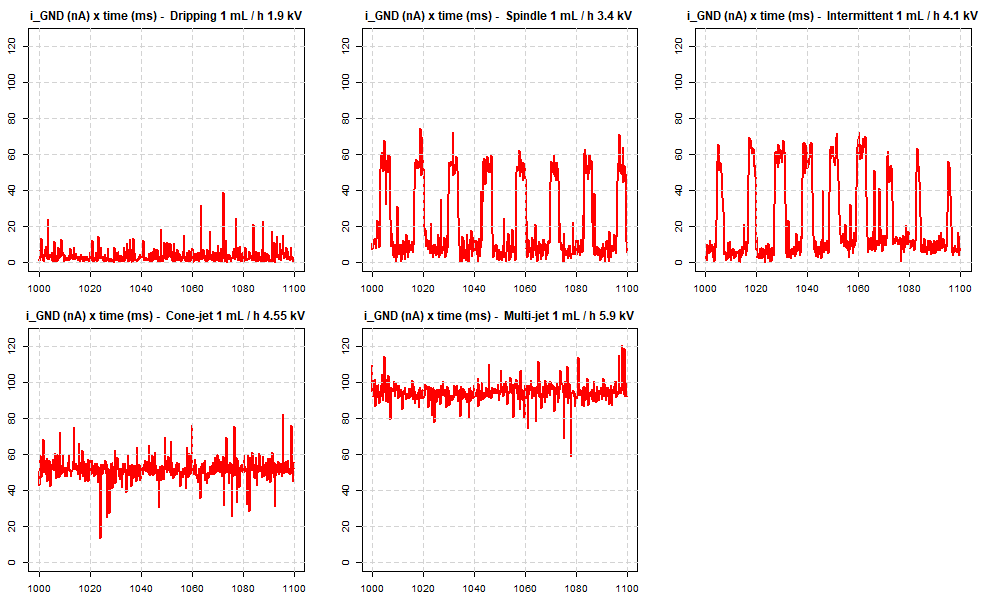
\includegraphics[width=1\textwidth,trim=1 1 1 1,clip]{figures/verdoold-reproduce-results.png}
    \caption{Results from the attempt to reproduce Verdoold's results on our setup.}
    \label{fig:verdoold-reproduce-results}
\end{figure}

As we can see in \autoref{fig:verdoold-reproduce-results}, we see a clear distinction between the spray modes, 
which is what we wish to see in the multinozzle. We can conclude that our measurement methodology can 
reproduce the results, therefore it must be something in the multinozzle that is "hiding" the intermittent spray 
signal.

Comparing the single nozzle setup on \autoref{fig:verdoold-reproduce-setup} and the multinozzle on \autoref{fig:setup-three-currents-spray-mode}, 
the most significant difference is indeed the presence of the crown. Therefore, let's begin by understanding the influence 
of the crown on $i_{GND}$, which is the current that we know is capable of showing a distinction of spraying 
modes. 

\subsection{Crown influences on $i_{GND}$}

To understad the influence of the crown on the ground current, we'll use the same setup shown on 
\autoref{fig:setup-three-currents-spray-mode}, but we'll make $V_+ = 0 \un{V}$, $\phi = 0 \un{mL / h}$ and measure $i_{GND}$ for different
crown voltages. Since there is no flow 
and no positive voltage, we'll be measuring the current on the groung ring introduced by the crown only.
In addition, we'll use coaxial cables during the measurements.

\autoref{fig:ignd-by-crown-no-filters} shows the shape of $i_{GND}$ for different values of $V_-$.

\begin{figure}[h!]
    \centering
    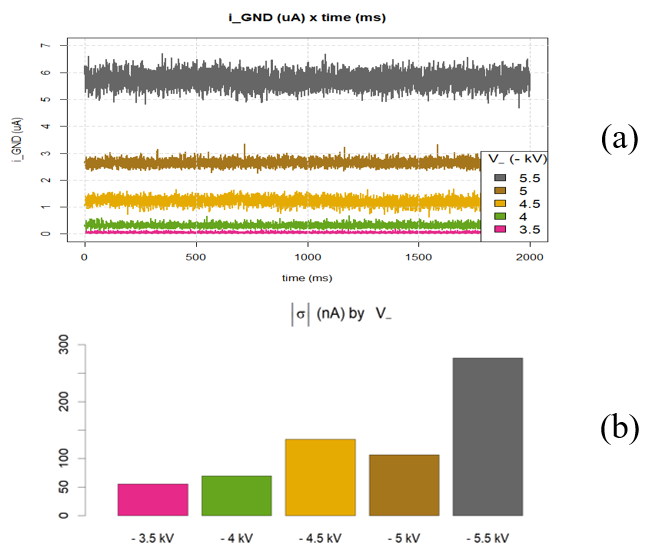
\includegraphics[width=1\textwidth,trim=1 1 1 1,clip]{figures/ignd-by-crown-no-filters.png}
    \caption{$i_{GND}$ for different values of $V_-$. (a) Waveform and (b) standard deviation}
    \label{fig:ignd-by-crown-no-filters}
\end{figure}

As seen of \autoref{fig:ignd-by-crown-no-filters} (a), the crown alone introduces a signal on $i_{GND}$ starting
from $V_- = - 4 \un{kV}$, which increases in both average value and standard deviation as $V_-$ increases.
This is consistent with was happens at the crown: from $V_- = - 4 \un{kV}$ onwards the sharp needles 
of the crown begin to ionize the air, producing ions that can be 
directed to ground ring. This results in a current $i_{GND} > 0$ induced by the crown.

In addition, on \autoref{fig:ignd-by-crown-no-filters} (b) we see that the standard deviation introduced by the crown
is significant. As we saw on \autoref{fig:verdoold-reproduce-results}, the intermittent spray mode 
presents peaks in the current signal in order of 50 nA, but the "noise" introduced by the 
crown alone is already over 50 nA when $V_- = -4.5 \un{kV}$, which is voltage used on the results 
of \autoref{fig:three-currents-spray-mode-500ms}. Therefore, it is reasonable to assume that the reason we are
not seing a good distinction between the spray modes on \autoref{fig:three-currents-spray-mode-500ms} is 
because of this signal introduced by the crown alone.

\subsubsection{Atenuating Crown Influences on $i_{GND}$}

In order to verify the above hypothesis, we can try to reduce the influence of the crown
in the signal and verify if the intermittent signal becomes distinguishable. We can achieve this adding digital filters 
in the oscilloscope software to remove the following frequencies:

\begin{itemize}
    \item 50 Hz frequency from the electric grid: use a stop band in the range 48 - 52 Hz
    \item All frequencies above 100 Hz: use low pass filter with cut-off frequency 100 Hz.
\end{itemize}

Since the intermittent peaks are usually under 100 Hz \citep{Verdoold2013}, we can remove 
anything above this frequency from the signal as it is not what we wish to measure.

Using this, we once again collect the signals of \autoref{fig:ignd-by-crown-no-filters}, obtaining the signal 
on \autoref{fig:ignd-by-crown-with-filters}.

\begin{figure}[h!]
    \centering
    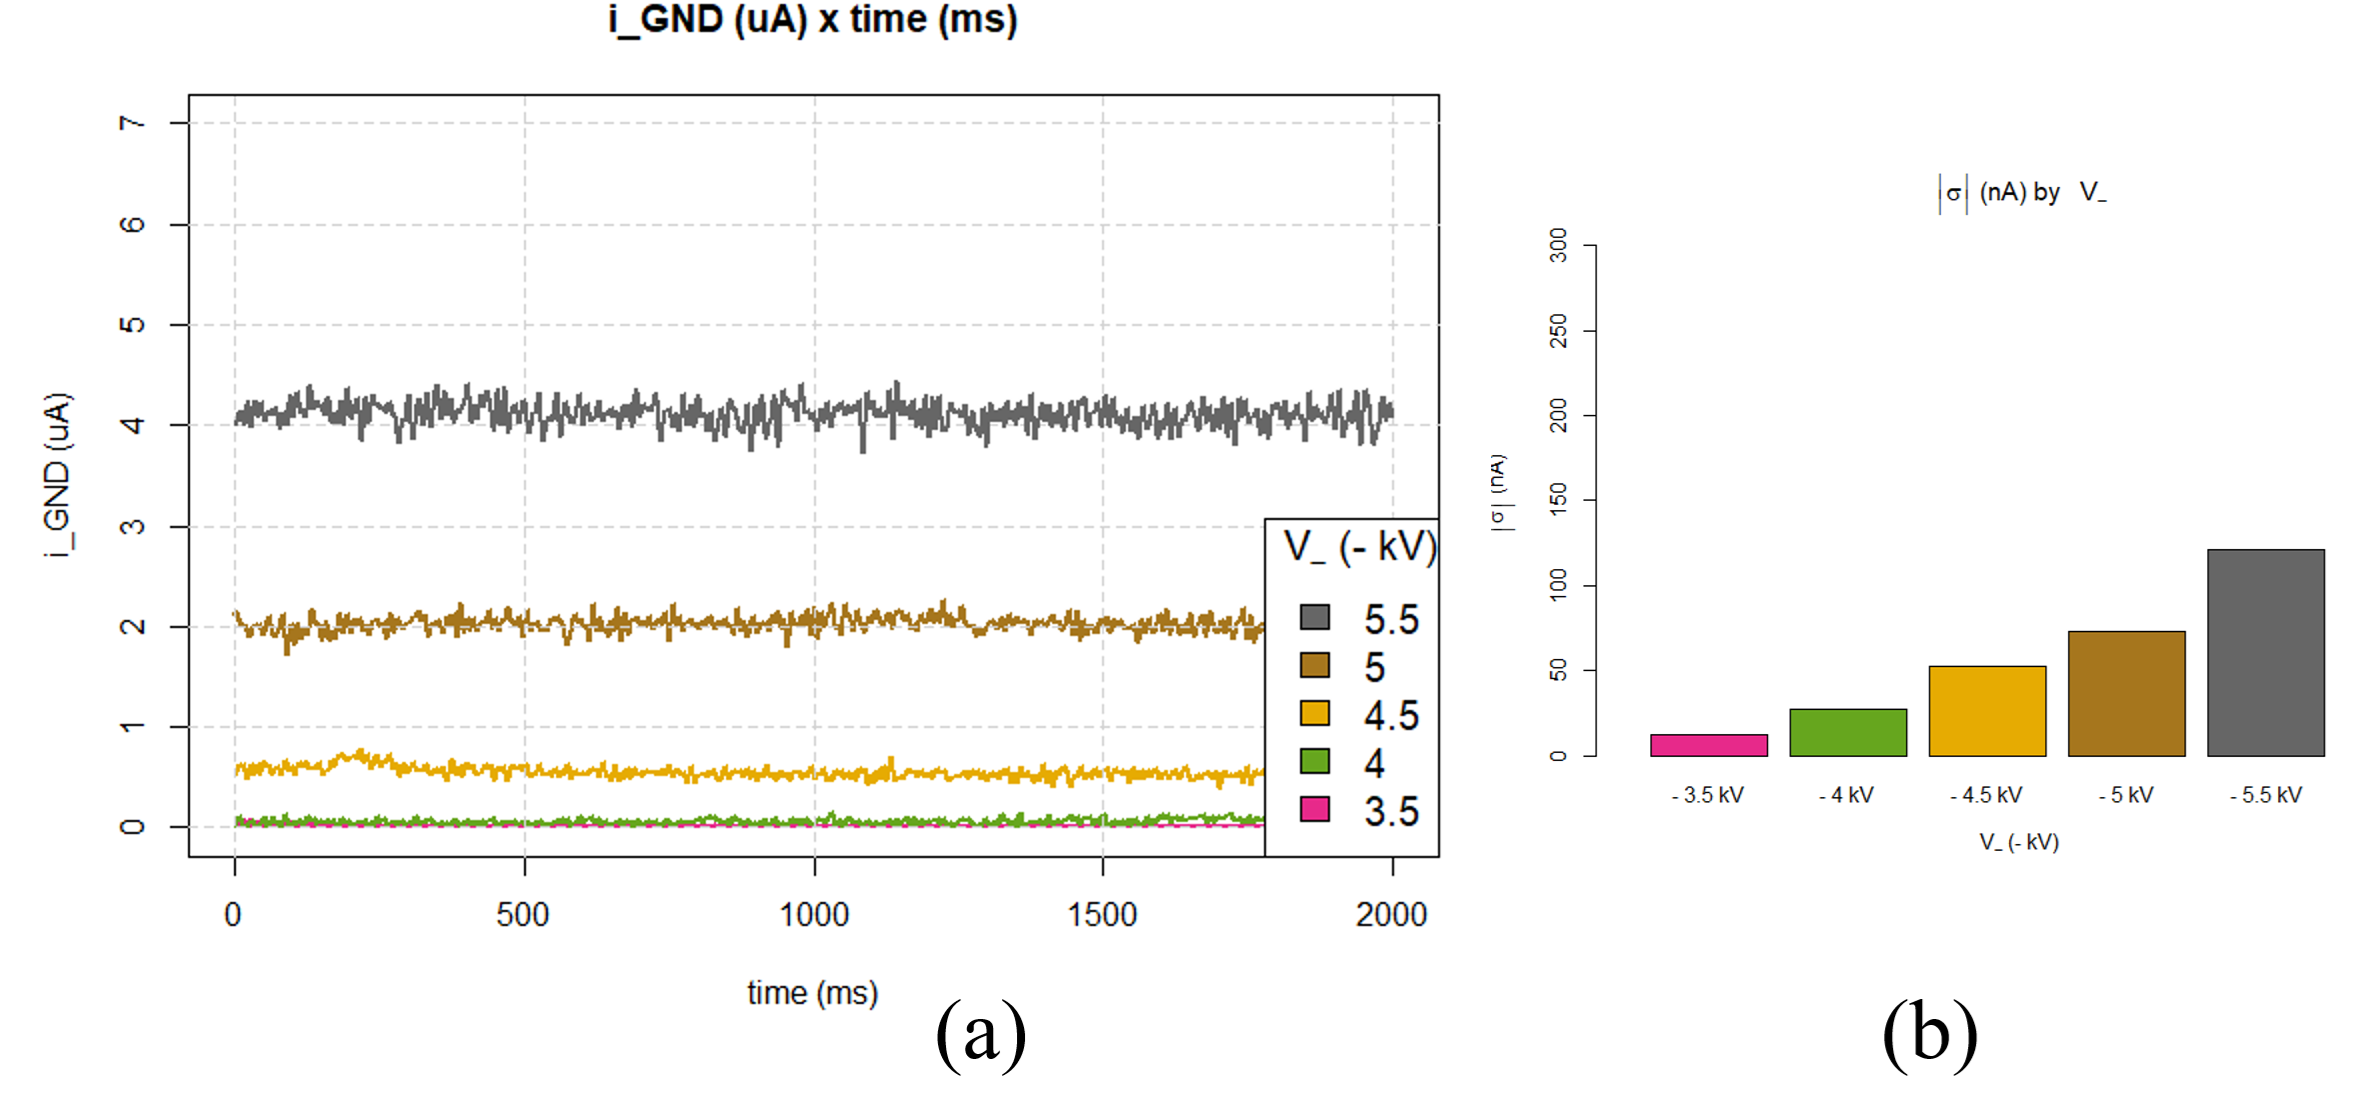
\includegraphics[width=1\textwidth,trim=1 1 1 1,clip]{figures/ignd-by-crown-with-filters.png}
    \caption{$i_{GND}$ for different values of $V_-$ with digital filters. (a) Waveform and (b) standard deviation}
    \label{fig:ignd-by-crown-with-filters}
\end{figure}

Comparing \autoref{fig:ignd-by-crown-with-filters} and \autoref{fig:ignd-by-crown-no-filters}, we see that the filters significantly 
reduce the standard deviation (i.e. the "noise") in $i_{GND}$. For $V_- = - 4.5 \un{kV}$, the standard deviation is already almost 
three times smaller. However, it remais above 50 nA, so it could still make it difficult to see the intermittent peaks in the signal.
Ideally, we would use the $V_- = - 4 \un{kV}$ to get the smallest amount of noise introduced, but it is not clear if it possible
to achieve a good neutralization with such a small $V_-$.

\subsubsection{8 vs 16 Needles in the Crown}

Around this time, Gilbert request us to test the crown with 8 needles for the WP2, as opposed to the 16 needles we had always used until 
this point. Difficulties to reinsert removed needles meant that from this point onwards we would always use a needle with 8 needles. 

Therefore, before we continue with this analysis, we need to understand how the signal introduces on $i_{GND}$ has changed. We've re-done 
the test of \autoref{fig:ignd-by-crown-with-filters}, obtaining the results shown on \autoref{fig:ignd-by-crown-8-needles}

\begin{figure}[h!]
    \centering
    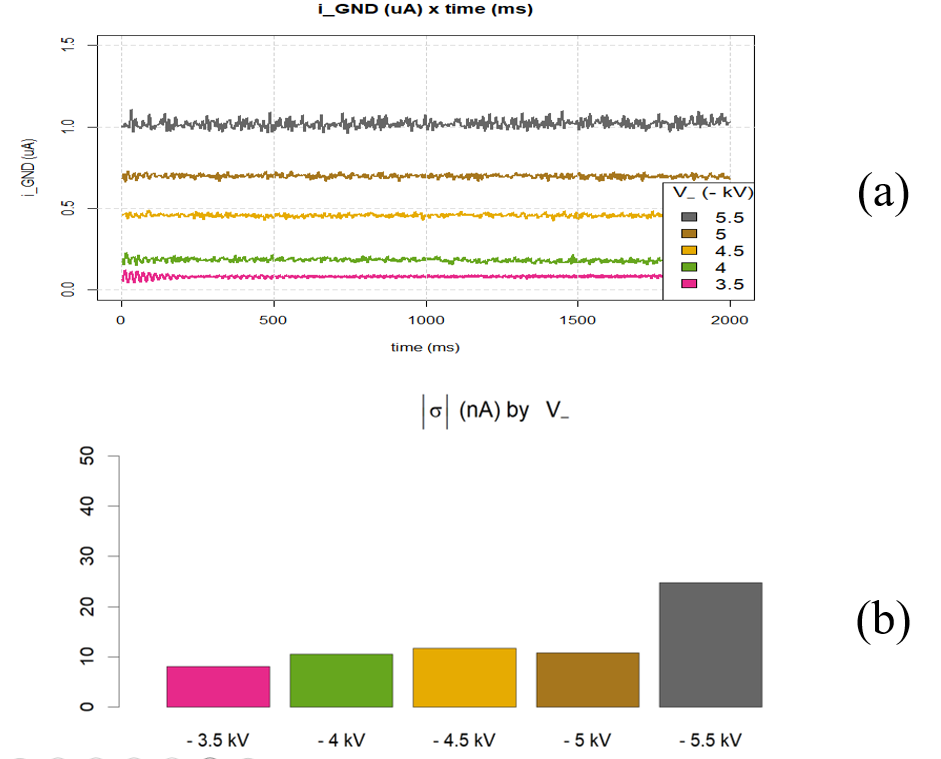
\includegraphics[width=1\textwidth,trim=1 1 1 1,clip]{figures/ignd-by-crown-8-needles.png}
    \caption{$i_{GND}$ for different values of $V_-$ with digital filters - Crown with 8 needles. (a) Waveform and (b) standard deviation}
    \label{fig:ignd-by-crown-8-needles}
\end{figure}

Comparing \autoref{fig:ignd-by-crown-with-filters} and \autoref{fig:ignd-by-crown-8-needles}, we see that the 8 needles introduce 
a much smaller signal on the $i_GND$, both in terms of average value as in standard deviation. This will be helpful to make  
the intermittent peaks on the signal more visible, as for $V_- = - 4.5 \un{kV}$ the introduced standard deviation is only 10 nA.

\subsection{Classifying the Spraying Mode}

With everything that we've now learned about the influence of the crown and the necessity of filters, we can now repeat the experiment 
of \autoref{fig:setup-three-currents-spray-mode}, using the same setup of \autoref{fig:setup-three-currents-spray-mode}, but again only
measuring $i_GND$. The oscilloscope was configured with $f_s = 5 \un{kHz}$ and a sample size of $N_s = 20.000$. The crown had 8 needles 
and was fixed with $V_- = - 4 \un{kV}$ to reduce as far as possible the influence of the crown on $i_GND$.

\autoref{fig:ignd-good-signal} shows the result obtained. The intermittent is clearly distinguishable from the cone-jet mode. However, 
expected, we cannot distinguish the elongated cone-jet and the multi-jet from the cone-jet.

\begin{figure}[h!]
    \centering
    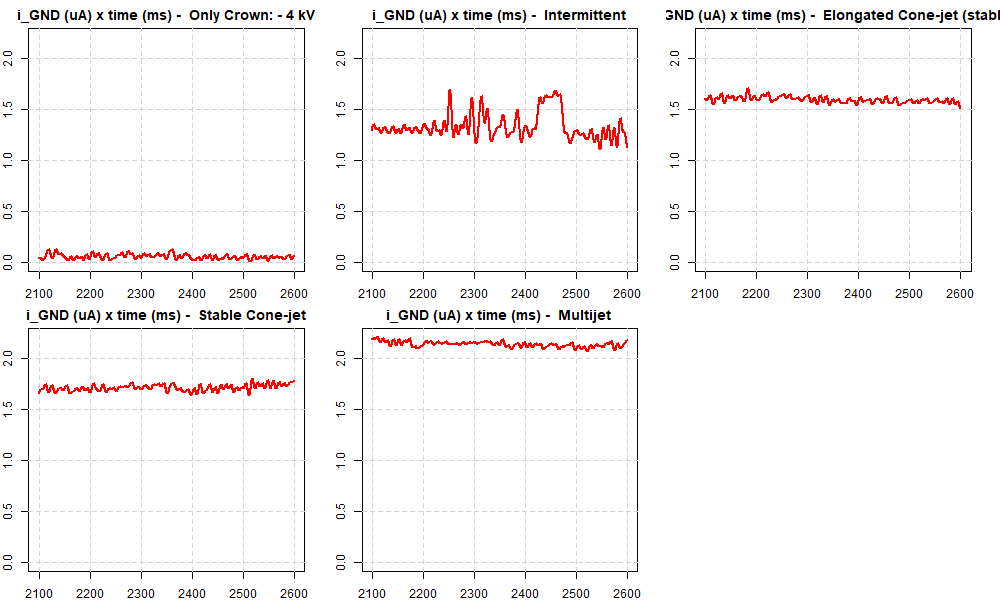
\includegraphics[width=1\textwidth,trim=1 1 1 1,clip]{figures/ignd-good-signal.png}
    \caption{$i_{GND}$ for different spray modes.}
    \label{fig:ignd-good-signal}
\end{figure}

Calculating the standard deviation on \autoref{fig:ignd-good-signal} also allows for a good distinction between the spraying modes,
as shown in \autoref{fig:ignd-good-sd}.

\begin{figure}[h!]
    \centering
    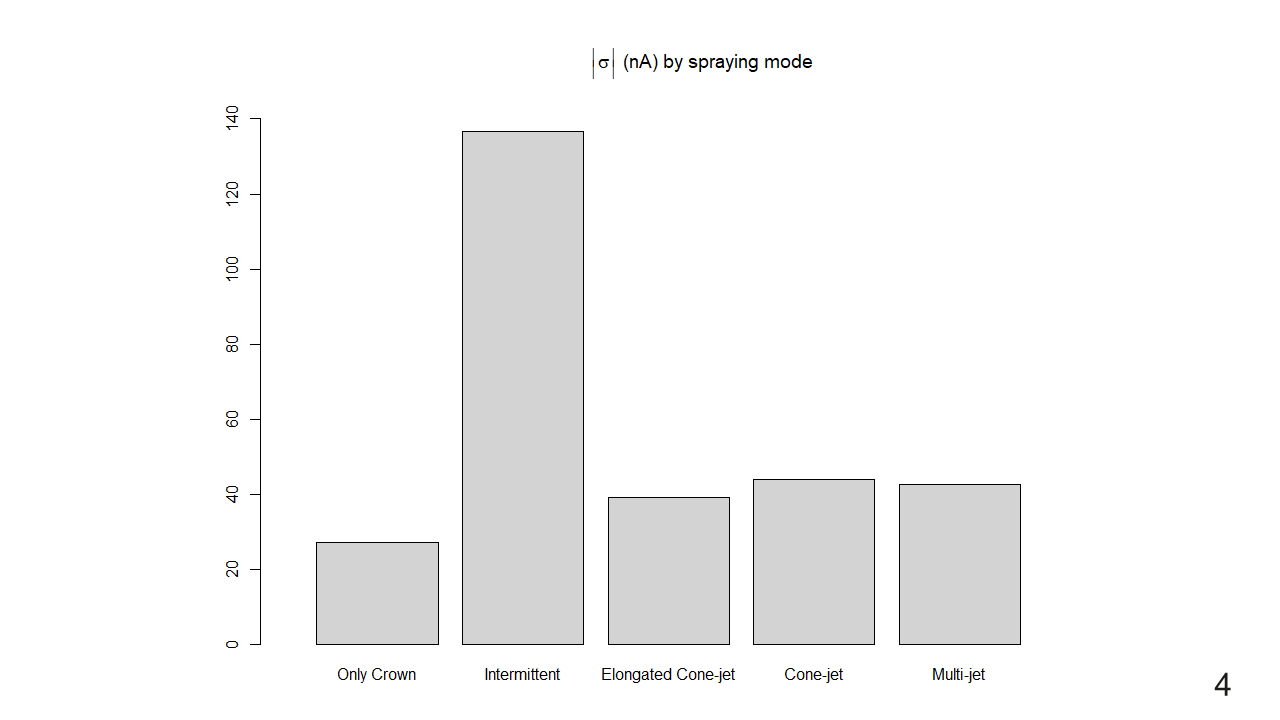
\includegraphics[width=1\textwidth,trim=1 1 1 1,clip]{figures/ignd-good-sd.png}
    \caption{Standard deviation of $i_{GND}$ for different spray modes.}
    \label{fig:ignd-good-sd}
\end{figure}

Based on \autoref{fig:ignd-good-sd}, we could use a simple if-else classification algorithm based on the standard deviation, 
defining a threshold for what is classified as intermittent or cone-jet. For example, we could say that if $\sigma > 60 \un{nA}$
then it is intermittent, else it is cone-jet (once inside the stable region defined by the mapping of the WP1).
An algorithm for this will be further explored on \autoref{sec:classification-algorithm}.


\subsection{Optimizing the Signal Acquisition}

In the previous sections, the signal was acquired using the minimum sampling frequency
suggested by the \cite{Verdoold2013} of $f_s = 5 \un{kHz}$. A sample size of $N_s = 20.000$ was used to obtain a spectral resolution of 0.25 Hz
for frequency domain anaysis, also suggested by Verdoold as the minimum. However, talks with Gilbert showed that the sampling frequency was too
computationally expensive and the sample size was too slow, as it resulted in a sampling time window of 4 seconds, which is too large.

Therefore, to attempt to meet these requirements, we need to find the minimum sampling frequency and
minimum sample size that can still reliably distinguish the signal of the intermittent from the cone-jet.

To do this, we'll use the following method:

\begin{itemize}
    \item Collect a time window of $T = 100$ seconds for different values of $f_s$, resulting in a sample size of $N_s = T \cdot f_s$
    \item Break the $T = 100$ seconds into smaller time windows - denoted as $S_i$ - of size $T_S$. 
    \item Calculate the relevant statistical parameters in each $S_i$ and store these values in an array of size $T / T_S$
    \item Plot a boxplot of the calculated statistical parameters
\end{itemize}

\autoref{fig:subsample-size-strategy} further explains the method above visually. $T_S$ will be chosen for different values for the result to be verified. 
Note that $i = 1, 2, ..., T / T_S$, and the goal is to find the minimum $T_S$.

\begin{figure}[h!]
    \centering
    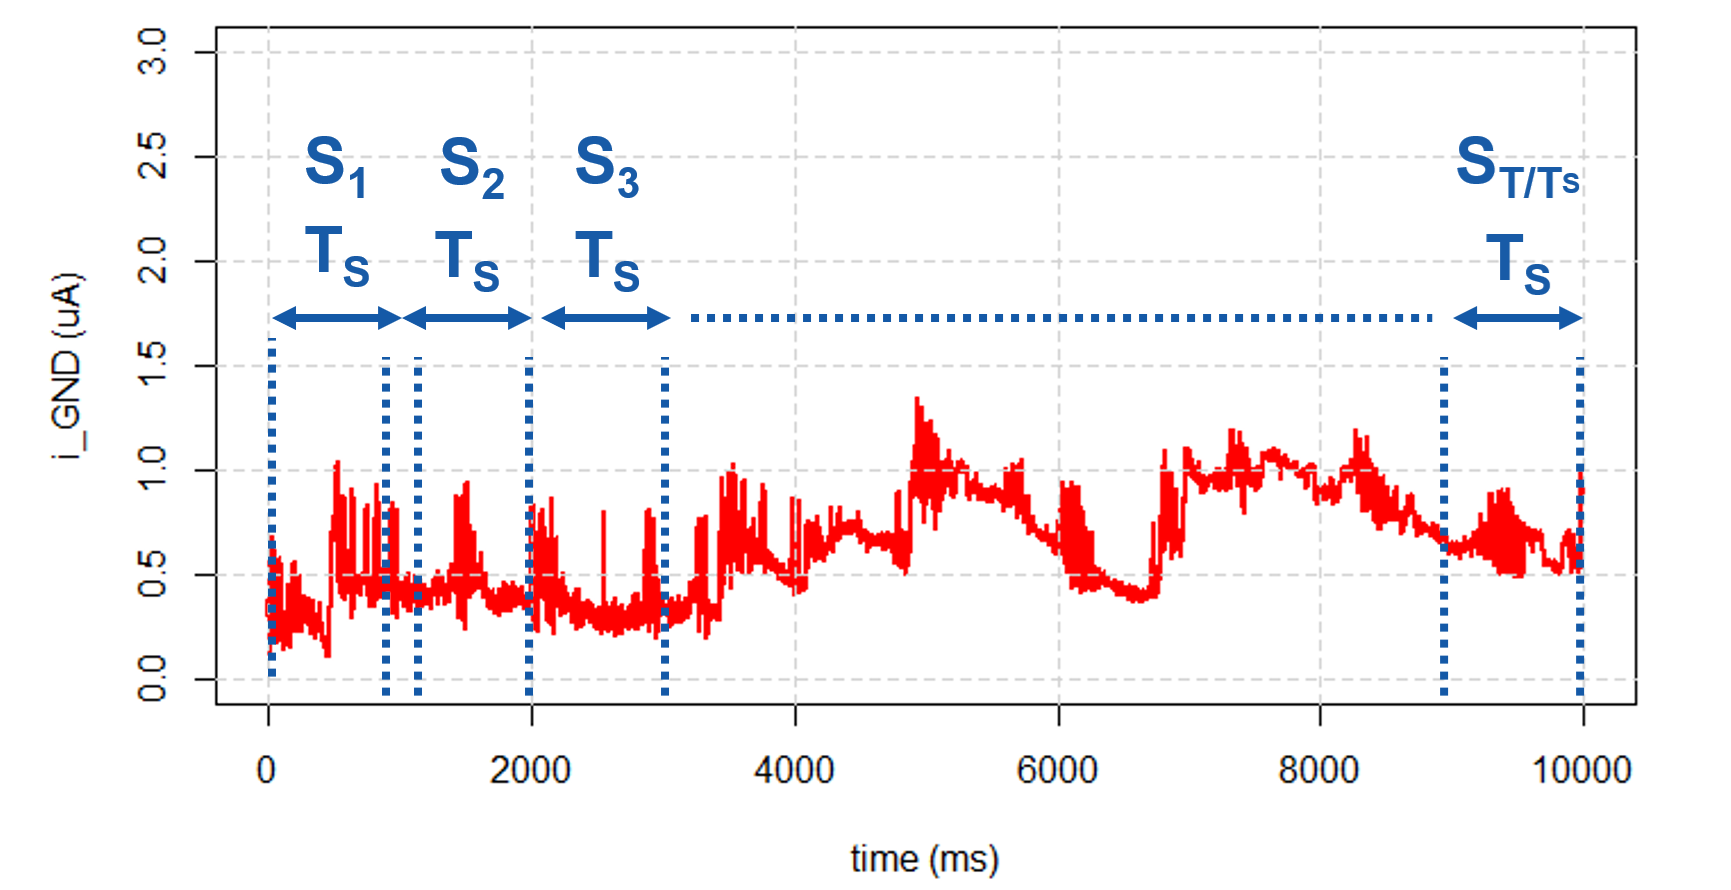
\includegraphics[width=.8\textwidth,trim=1 1 1 1,clip]{figures/subsample-size-strategy.png}
    \caption{Method to find the minimum sample size that can still classify the EHDA mode via the current.}
    \label{fig:subsample-size-strategy}
\end{figure}

We'll use the same setup shown in \autoref{fig:setup-three-currents-spray-mode}, using only the oscilloscope for $i_{GND}$.
We begin with $f_s = 5 \un{kHz}$, with $T_S = 0.01 \un{s}; 0.1 \un{s}; 1 \un{s}; 10 \un{s}$. Note that we are first changing
$T_S$ over four orders of magnitude to understand the general influence of $T_S$ on the calcualated standard deviation.
The result obtained is shown on \autoref{fig:first-test-subsample}.

\begin{figure}[h!]
    \centering
    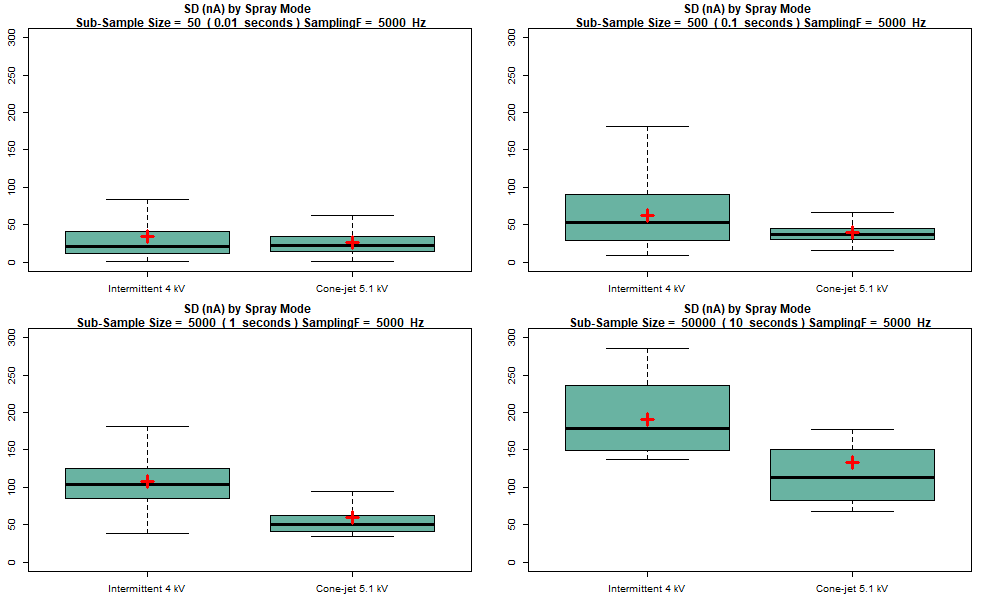
\includegraphics[width=\textwidth,trim=1 1 1 1,clip]{figures/first-test-subsample.png}
    \caption{Calculated standard deviation for $f_s = 5 \un{kHz}$, with $T_S = 0.01 \un{s}; 0.1 \un{s}; 1 \un{s}; 10 \un{s}$}
    \label{fig:first-test-subsample}
\end{figure}

As we can see on \autoref{fig:first-test-subsample}, $T_S = 1 \un{s}$ appears to be the best sample size to 
differentiate between the intermittent and the cone-jet. Other orders of magnitude of $T_S$ do not allow for a clear distinction
between spraying mode via the statistical values. The next test is to change $T_S$ around 1 second and compare them, 
using $T_S = 0.25 \un{s}; 0.5 \un{s}; 0.75 \un{s}; 1 \un{s}$. \autoref{fig:second-test-subsample} shows the results obtained  
for this test.

\begin{figure}[h!]
    \centering
    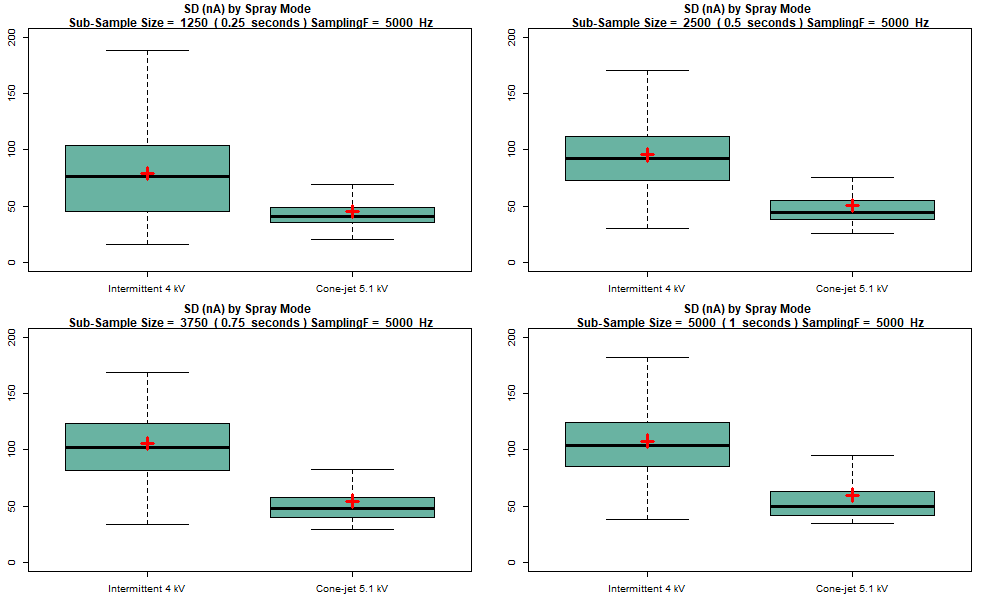
\includegraphics[width=\textwidth,trim=1 1 1 1,clip]{figures/second-test-subsample.png}
    \caption{Calculated standard deviation for $f_s = 5 \un{kHz}$, with $T_S = 0.25 \un{s}; 0.5 \un{s}; 0.75 \un{s}; 1 \un{s}$}
    \label{fig:second-test-subsample}
\end{figure}

As seen on \autoref{fig:second-test-subsample}, $T_S = 0.5 \un{s}$ appears to be the smallest sample size that can differentiate the spraying modes.
$T_S = 0.5 \un{s}$ may still be feasible, but it presents significant overlapping between the two modes around $\sigma = 50 \un{nA}$.

Now we need to find the minimum sampling frequency that can distinguish the spraying modes. We'll fix $T_S = 0.5 \un{s}$ and compare the calculated 
statistical parameters for the following values of $f_s$: $f_s = 0.5 \un{kHz}; 1 \un{kHz}; 2 \un{kHz}; 5 \un{kHz}$. \autoref{fig:third-test-subsample}
shows the result obtained for this test.

\begin{figure}[h!]
    \centering
    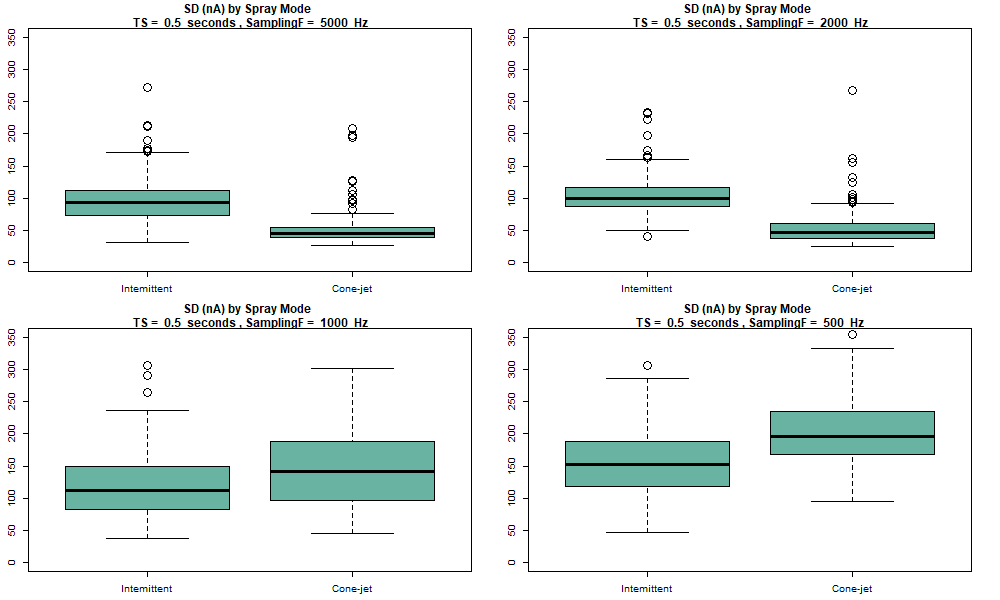
\includegraphics[width=1\textwidth,trim=1 1 1 1,clip]{figures/third-test-subsample.png}
    \caption{Calculated standard deviation for $T_s = 0.5 \un{s}$, with $f_s = 0.5 \un{kHz}; 1 \un{kHz}; 2 \un{kHz}; 5 \un{kHz}$}
    \label{fig:third-test-subsample}
\end{figure}

As we can see on \autoref{fig:third-test-subsample}, $f_s = 2 \un{kHz}$ appears to the be the smallest sampling frequency that can still distinguish the spraying  
modes. 

The conclusion we can derive from these tests is that $T_S = 0.5 \un{s}$ and $f_s = 2 \un{kHz}$ are the mininum sample size and sampling frequency that
can distinguish the spraying modes via statistical parameters. Note that this results in a sample size of $N_s = T_S f_s = 1.000$, which uses 
significantly less memory than the $N_s = 20.000$. We'll move forward with these values of $N_s$ and $f_s$, seeking to test the classification
with parameters that are consistent with Gilbert's requirements.

\subsection{Optimizing the Classification}

\subsubsection{Trying different statistical parameters}

So far, we've only the standard deviation of the signal to differentiate the spraying modes. However, we can also use other statistical parameters 
to distinguish the waveforms. The first one that we can try is the Relative Standard Deviation (RSD), defined on \autoref{eq:rsd}


\begin{equation} \label{eq:rsd}
    RSD = \left|\frac{\sigma}{\overline{I}}\right|
\end{equation}

where

\begin{itemize}
    \item $\sigma$: standard deviation
    \item $\overline{I}$: arithmetic mean
\end{itemize}

\autoref{tab:rsd} shows how the RSD can be a useful metric in the classification. When the spraying mode is intermittent, we 
expect the signal to display a large $\sigma$ and a small $\overline{I}$, since the potential is lower and therefore also the mean value 
of the current in the system. This results in an overall value large value of the ratio. 

\begin{table}[h!]
    \begin{center}
      \caption{Expected behaviour of RSD for different spraying modes.}
      \label{tab:rsd}
      \begin{tabular}{c|c|c}
        \textbf{} & \textbf{Intermittent} & \textbf{Cone-jet}\\
        \hline
        Numerator ($\sigma$) & HIGH & LOW\\
        Denominator ($\overline{I}$) & LOW& HIGH\\
        Overall Ratio ($\sigma / \overline{I}$) & LARGE & SMALL\\
      \end{tabular}
    \end{center}
  \end{table}

On the other hand, when we have a cone-jet, we expect the signal to display a small $\sigma$ - as the signal is much more stable -
and a larger $\overline{I}$, given the larger potential. This results in an overall value small value of the ratio.

Therefore, both components of the fraction contribute in opposite directions to change the overall value of the ratio between the spraying modes,
making this metric a potentially good classification parameter.

\autoref{fig:rsd-subsample} shows the the same result of \autoref{fig:third-test-subsample} using the RSD instead of the standard deviation.

\begin{figure}[h!]
    \centering
    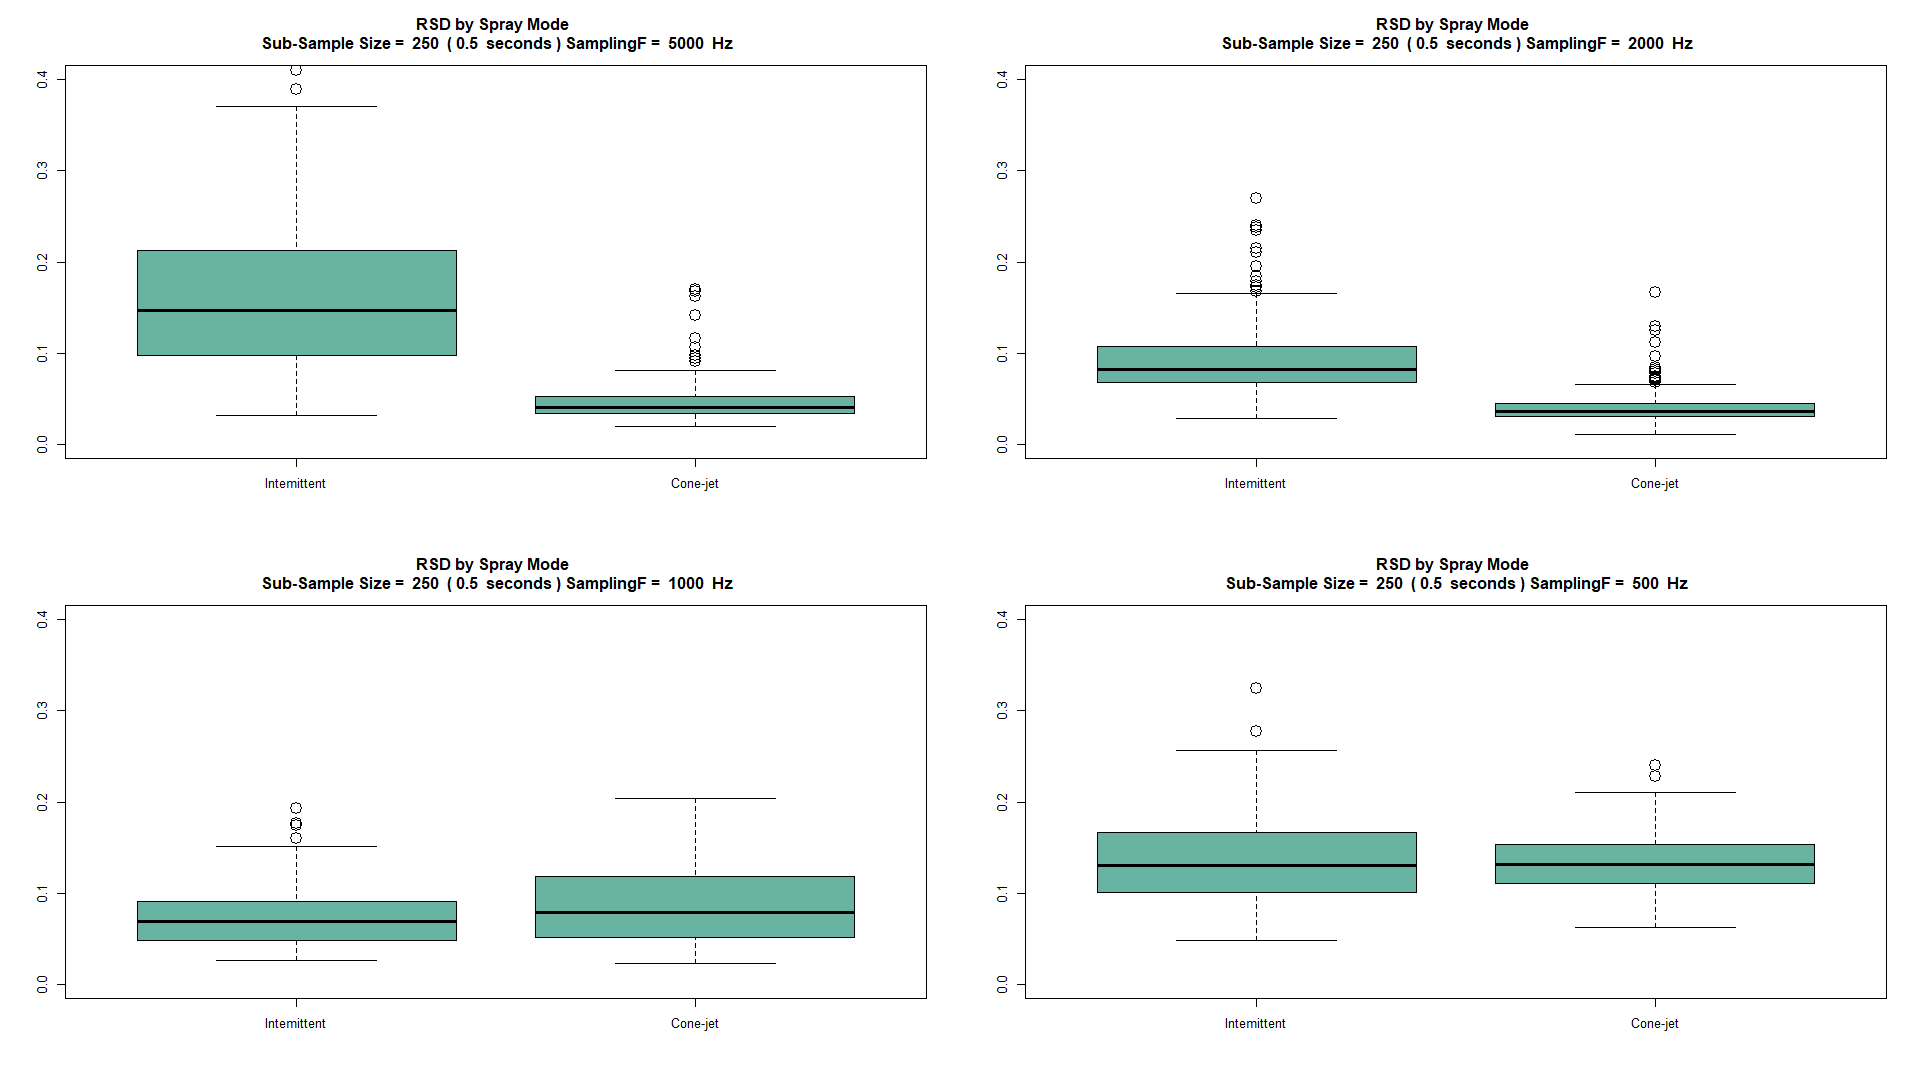
\includegraphics[width=\textwidth,trim=1 1 1 1,clip]{figures/rsd-subsample.png}
    \caption{Calculated RSD for $T_s = 0.5 \un{s}$, with $f_s = 0.5 \un{kHz}; 1 \un{kHz}; 2 \un{kHz}; 5 \un{kHz}$}
    \label{fig:rsd-subsample}
\end{figure}

As we can see on \autoref{fig:rsd-subsample}, we can achieve a good distinction between the spraying modes with the RSD. However, the 
order of magnitude of the value is very small, which can be inconvenient. A simple to resolve this is take the inverse of the RSD, that 
we can define as the Signal-to-Noise Ratio (SNR), shown on \autoref{eq:snr}

\begin{equation} \label{eq:snr}
    SNR = \frac{1}{RSD} = \left|\frac{\overline{I}}{\sigma}\right|
\end{equation}

In \autoref{eq:snr}, we call the standard deviation as the "noise", and the mean as the "signal". \autoref{fig:snr-subsample} shows the
same result of \autoref{fig:third-test-subsample} using the SNR.

\begin{figure}[h!]
    \centering
    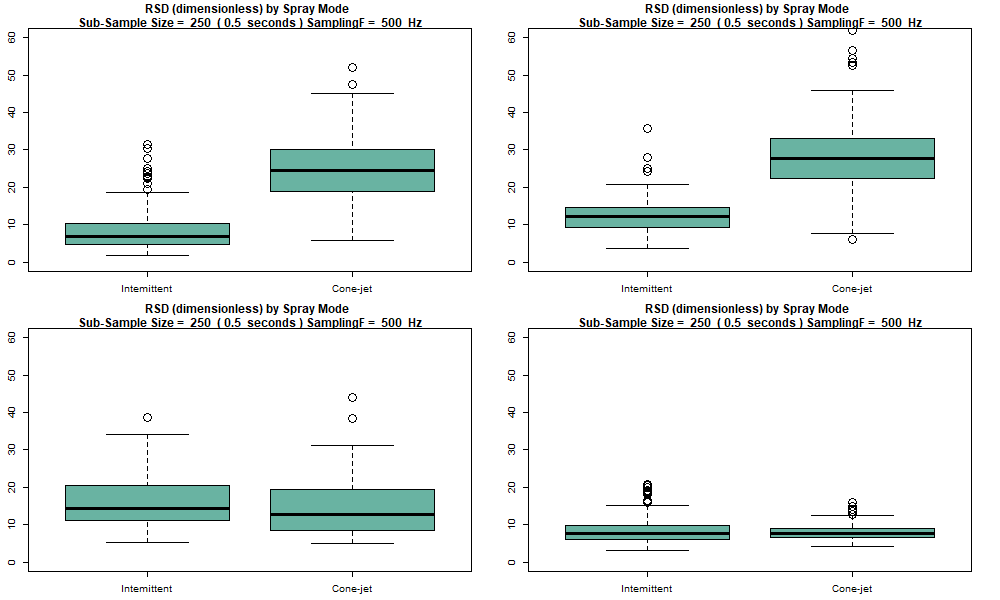
\includegraphics[width=\textwidth,trim=1 1 1 1,clip]{figures/snr-subsample.png}
    \caption{Calculated SNR for $T_s = 0.5 \un{s}$, with $f_s = 0.5 \un{kHz}; 1 \un{kHz}; 2 \un{kHz}; 5 \un{kHz}$}
    \label{fig:snr-subsample}
\end{figure}

As seen on \autoref{fig:snr-subsample}, the SNR is also a good metric to distinguish the intermittent and cone-jet modes.
Unlike the RSD, the SNR spreads from the range 0 - 50, making it more convenient that the RSD and showing less outliers. 
Therefore, the RSD will be used from this point on, using $f_s = 2 \un{kHz}$ and $N_s = 1.000 \quad (T_S = 0.5 \un{s})$. 

\subsubsection{Classification via small Neural Networks}

\hl{ASK BEN}

\subsection{Proof-of-Concept Real-time EHDA Classification}\label{sec:classification-algorithm}

TODO
\begin{itemize}
    \item try to reduce sample window
    \item use subsequent windows
    \item show commmon issues (step in the current value, etc)
    \item add pseudocode + complexity
\end{itemize}

\subsection{Proof-of-Concept Real-Time EHDA Control}
TODO

\begin{itemize}
    \item problem wth subsequent window: how will it take into account the adjusts we're making:
    \item is it fast enough? if it even works at all!
    \item add pseudocode + complexity
\end{itemize}

% ==============================================
\newpage    \pagestyle{plain}
\addcontentsline{toc}{chapter}{References} % 'References' will appear in the index.
\bibliography{references.bib}
% ==============================================
\end{document}